\documentclass{article}
\usepackage{graphicx}
\usepackage{amsmath}
\usepackage{amssymb}
\usepackage[T1]{fontenc}
\usepackage[utf8]{inputenc}
\usepackage[polish]{babel}

\title{PythonKrakowski}
\author{Arkadiusz Wzorek, Zofia Ficek, Mikołaj Mazur, Bartosz Pieczek}
\date{October 2024}

\begin{document}

\maketitle

\tableofcontents % Spis treści

\newpage

\section{Wstęp}

Każdy z autorów przygotuje osobny rozdział, który będzie zawierał różnorodne elementy takie jak na przykład:
\begin{itemize}
    \item Wyrażenie matematyczne,
    \item Zdjęcie,
    \item Tabelę,
    \item Listę numerowaną,
    \item Listę nienumerowaną.
\end{itemize}

\newpage

\section{Bartosz Pieczek}

\subsection{Albert Einstein i $E = mc^2$}

\hspace{\parindent}Albert Einstein jest najbardziej znany ze swojej teorii względności, zawartej w równaniu \( E = mc^2 \), które zrewolucjonizowało fizykę.\par\textbf{Albert Einstein} wprowadził nową perspektywę na \textbf{masę} i \textbf{energię}, pokazując, że są one \textit{równoważne}. Jego równanie stało się \textbf{fundamentem} współczesnej fizyki i wpłynęło na rozwój technologii, takich jak \textit{energia jądrowa}.


\subsection{Wyrażenie matematyczne}
Energia (\( E \)) obiektu jest związana z jego masą (\( m \)) oraz prędkością światła (\( c \)) według wzoru:
\[
E = mc^2
\]

\subsection{Obraz}
Na rysunku \ref{fig:einstein} przedstawiono znane zdjęcie Alberta Einsteina.

\begin{figure}[ht]
    \centering
    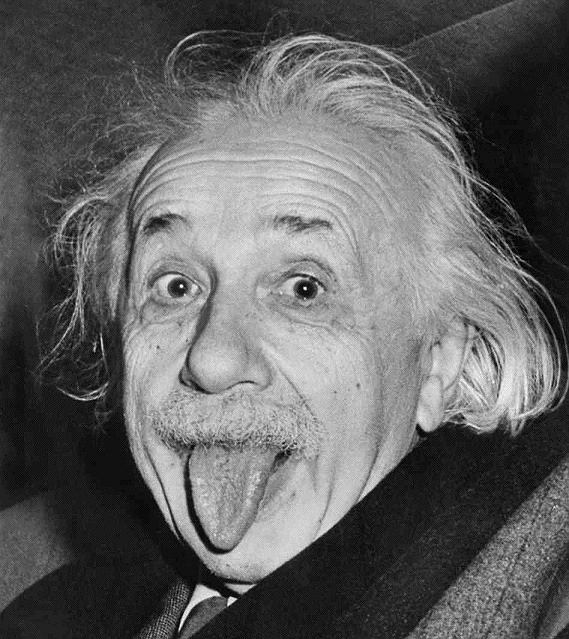
\includegraphics[width=0.5\textwidth]{pictures/einstein.jpg}
    \caption{Albert Einstein}
    \label{fig:einstein}
\end{figure}

\subsection{Lista numerowana:}
Przykład listy numerowanej:
\begin{enumerate}
    \item Albert Einstein urodził się w 1879 roku.
    \item Opracował teorię względności.
\end{enumerate}

\subsection{Tabela}
Tabela \ref{tab:mass-energy} przedstawia wartości związane z równaniem masy i energii.

\begin{table}[ht]
    \centering
    \begin{tabular}{|c|c|}
    \hline
    Masa (kg) & Energia (J) \\ \hline
    $1$        & $8.99 \times 10^{16}$ \\ \hline
    $10$       & $8.99 \times 10^{17}$ \\ \hline
    \end{tabular}
    \caption{Tabela masy i energii}
    \label{tab:mass-energy}
\end{table}


\subsection{Lista nienumerowana:}
I lista nienumerowana z pauzami:
\begin{itemize}
    \renewcommand\labelitemi{--}
    \item Równanie \( E = mc^2 \) zmieniło nasze rozumienie energii.
    \item Zasada ta dotyczy każdej materii.
\end{itemize}
\pagebreak
\section{Arkadiusz Wzorek}
\label{sec:awzorek}

\subsection{Leonhard Euler}

\textbf{Leonhard Euler} – szwajcarski matematyk i fizyk; był pionierem w wielu obszarach obu tych nauk. Jest uważany za czołowego matematyka XVIII wieku i jednego z najwybitniejszych w całej historii. Euler wniósł wkład do niemal wszystkich ówczesnych dziedzin matematyki:

\begin{itemize}
    \item[--] geometrii,
    \item[--] rachunku różniczkowego i całkowego,
    \item[--] trygonometrii,
    \item[--] algebry,
    \item[--] teorii liczb.
\end{itemize}

\noindent Poniżej (rysunek \ref{fig:euler}) portret uczonego:

\begin{figure}[htbp]
    \centering
    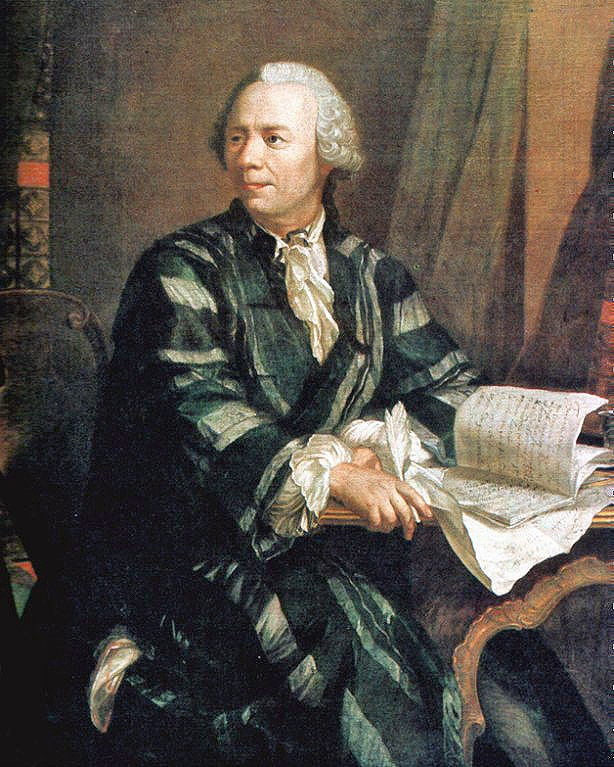
\includegraphics[width=0.5\textwidth]{pictures/euler.jpg}
    \caption{Leonhard Euler.}
    \label{fig:euler}
\end{figure}

\subsection{Wzór Eulera}

\textbf{Wzór Eulera} – wzór analizy zespolonej wiążący funkcje trygonometryczne z zespoloną funkcją wykładniczą, określany nazwiskiem Leonharda Eulera.

Niech $ x\in\mathbb{R} $, zaś $ i $ jest jednostką urojoną, wtedy wzór Eulera ma postać:
$$ e^{ix} = \cos x + i\sin x $$

\subsection{„Najpiękniejszy wzór”}
W szczególności, podstawiając $ x = \pi $, otrzymuje się równość:
$$ e^{\pi i} + 1 = 0 $$
nazywaną \textbf{tożsamością Eulera}.

Tożsamość Eulera nazywana jest często \textit{najpiękniejszym wzorem matematycznym}. Wykorzystane są w niej trzy działania arytmetyczne: dodawanie, mnożenie i potęgowanie. Tożsamość łączy pięć fundamentalnych stałych matematycznych:

\begin{enumerate}
    \item liczbę 0,
    \item liczbę 1,
    \item liczbę $ \pi $,
    \item liczbę $ e $,
    \item liczbę $ i $, jednostkę urojoną liczb zespolonych.
\end{enumerate}

Dodatkowo każde z powyższych działań oraz każda ze stałych użyte są \textit{dokładnie raz}, co więcej: wzór ten jest przedstawiony w zwyczajowej formie równania, którego prawa strona jest zerem.

\subsection{Inne szczególne przypadki}

Tabela \ref{tab:special_cases} przedstawia pozostałe ciekawe przypadki wzoru Eulera.

\begin{table}[htbp]
    \centering
    \begin{tabular}{|c|c|}
        \hline
        $ x $ & $ e^{ix} $ \\
        \hline
        $ 0 + 2k \pi$ & $ 1 $ \\
        \hline
        $ \frac{\pi}{2} + 2k \pi $ & $ i $ \\
        \hline
        $ \pi + 2k \pi $ & $ -1 $ \\
        \hline
        $ \frac{3\pi}{2} + 2k \pi $ & $ -i $ \\
        \hline
    \end{tabular}
    \caption{Inne szczególne przypadki wzoru Eulera.}
    \label{tab:special_cases}
\end{table}
\pagebreak
\input{chapters/MikołajMazur}
\pagebreak
\section{Zofia Ficek}

\subsection{Carl Friedrich Gauss}

\hspace{\parindent} \textbf{Carl Friedrich Gauss} był niemieckim matematykiem, urodzonym w 1777 roku. Już w dzieciństwie wykazywał niezwykłe zdolności matematyczne, co zaowocowało jego późniejszymi osiągnięciami. Jego najważniejszym dziełem jest \textit{"Disquisitiones Arithmeticae"}, które zrewolucjonizowało teorię liczb. 
\par \textbf{Gauss} wprowadził pojęcie kongruencji oraz zajmował się badaniem liczb pierwszych. Jego prace w analizie matematycznej przyczyniły się do rozwoju teorii funkcji i równań różniczkowych. Znany jest również z analizy statystycznej, w tym z wprowadzenia rozkładu normalnego, zwanego krzywą Gaussa. Gauss zmarł w 1855 roku, pozostawiając po sobie niezatarte ślady w matematyce i nauce.
\par\noindent Poniżej (Rysunek \ref{fig:gauss}) portret uczonego
\begin{figure}[ht]
    \centering
    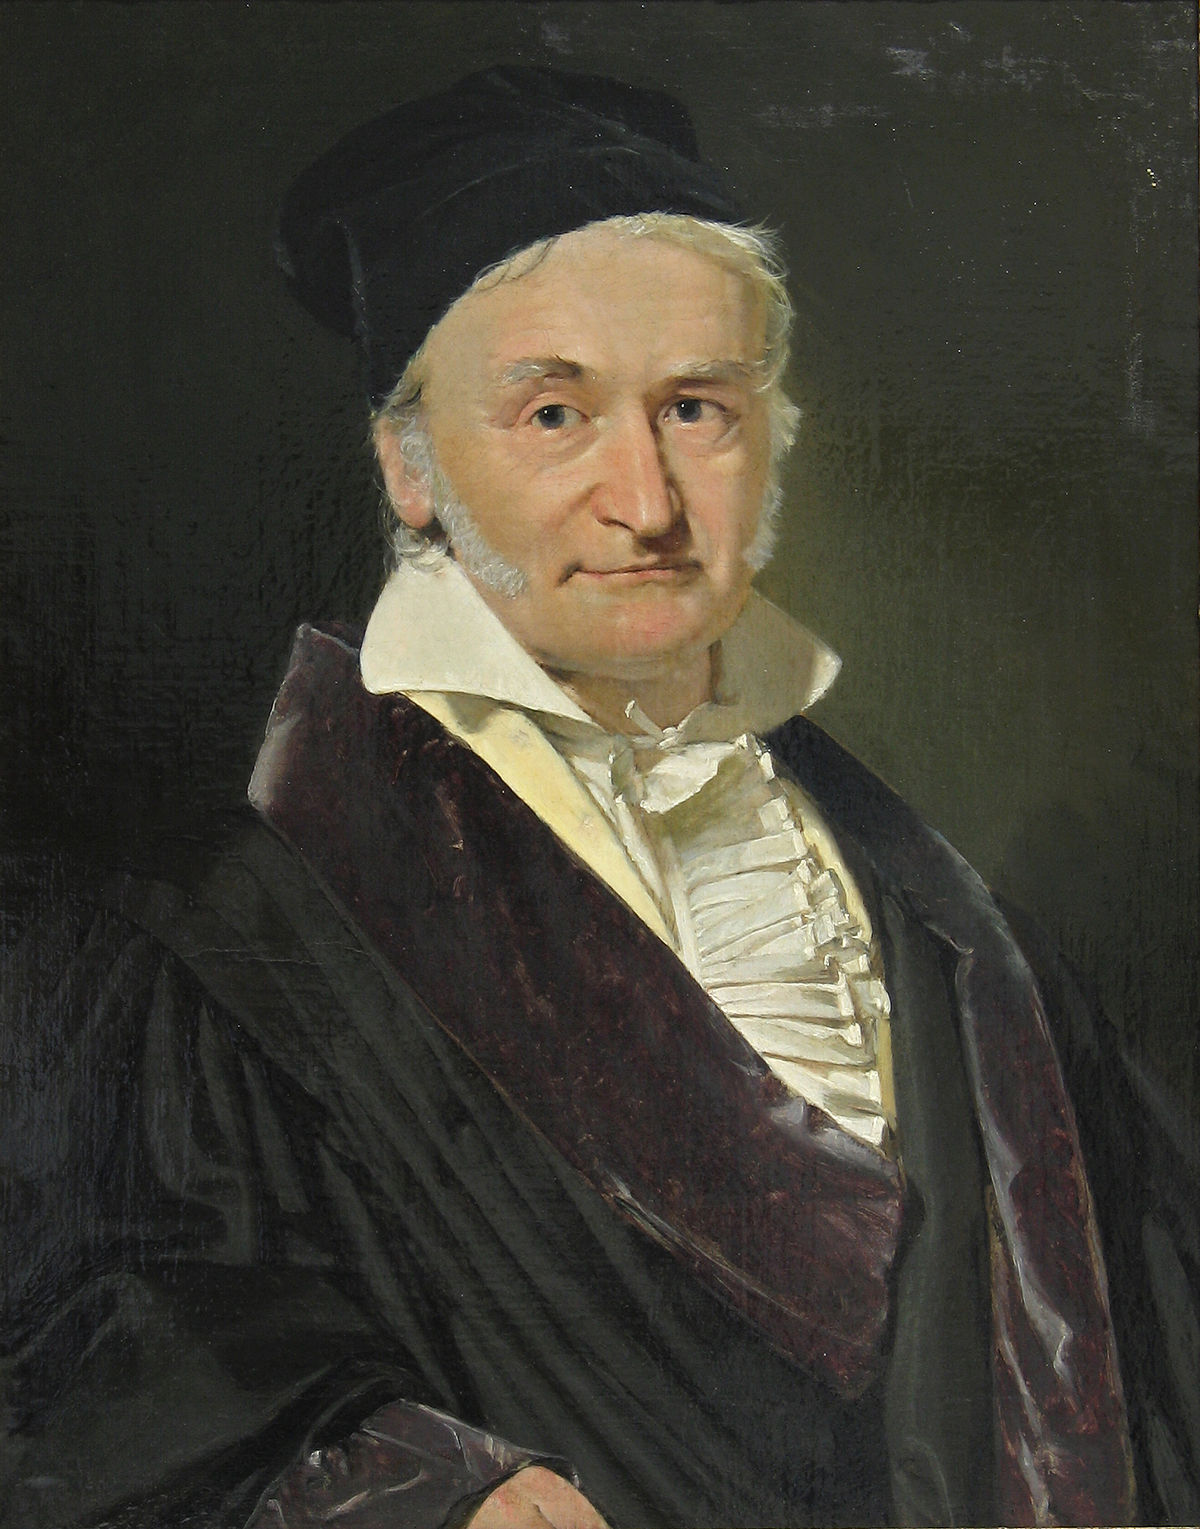
\includegraphics[width=0.5\textwidth]{pictures/gauss.jpg}
    \caption{Carl Friedrich Gauss}
    \label{fig:gauss}
\end{figure}

\subsection{Krzywa Gaussa}
\hspace{\parindent} \textbf{Krzywa Gaussa}, znana również jako krzywa normalna, to graficzne przedstawienie rozkładu normalnego. Jest to jeden z najważniejszych rozkładów w statystyce, charakteryzujący się symetrią i dzwonowatym kształtem
\par \textbf {Wzór krzywej Gaussa}, jest dany przez
\[f(x) = \frac{1}{\sigma \sqrt{2\pi}} e^{-\frac{(x - \mu)^2}{2\sigma^2}}\]
\begin{itemize}
    \renewcommand\labelitemi{--}
    \item $f(x)$ to wartość funkcji gęstości rozkładu dla punktu $x$
    \item \( \mu\) to średnia rozkładu
    \item \(\sigma\) to odchylenie standardowe
    \item $e$ to podstawa logarytmu naturalnego (około 2.71828)
    \item \(\pi\) to liczba Pi (około 3.14159)
\end{itemize}
\vspace{0,5cm} 
\par Kluczowe cechy \textbf{krzywej Gaussa}
\begin{enumerate}
    \item \textbf{Symetria}: Krzywa jest symetryczna względem swojej średniej, co oznacza, że wartości są równomiernie rozłożone po obu stronach.
    \item \textbf{Średnia, mediana, dominanta}: W rozkładzie normalnym te trzy miary centralne są sobie równe i znajdują się w punkcie szczytu krzywej.
    \item \textbf{Parametry}: Krzywa Gaussa jest określona przez dwa parametry: średnią \( \mu\) i odchylenie standardowe \(\sigma\). Średnia wskazuje, gdzie znajduje się środek rozkładu, a odchylenie standardowe określa, jak bardzo dane są rozproszone.
    \item \textbf{Zastosowania}: Powszechnie używana w statystyce, naukach przyrodniczych, ekonomii i wielu innych dziedzinach do modelowania danych i zjawisk losowych.
\end{enumerate}

\subsection{Nagroda Gaussa}
\par Nagroda Gaussa (Nagroda im. Carla Friedricha Gaussa) to prestiżowe wyróżnienie przyznawane przez Międzynarodową Unię Matematyczną (IMU) za wybitne osiągnięcia w dziedzinie matematyki. Nagroda jest często uważana za równoważną z innymi prestiżowymi wyróżnieniami w dziedzinie nauk, takimi jak Nagroda Nobla. Tabela \ref{tab:gauss} przedstawia daty i zdobywców Nagrody Gaussa:
\begin{table}[ht]
    \centering
    \begin{tabular}{|c|c|}
    \hline
    Rok & Zdobywca nagrody              \\
    \hline
    2006 & Jean-Pierre Serre            \\
    \hline
    2007 & S. R. Srinivasa Varadhan     \\
    \hline
    2008 & John G. Thompson             \\
    \hline
    2009 & Mikio Sato                   \\
    \hline
    2010 & John Nash                    \\
    \hline
    2011 & Goro Shimura                 \\
    \hline
    2012 & Alain Connes                 \\
    \hline
    2013 & Peter Scholze                \\
    \hline
    2014 & Andrew Wiles                 \\
    \hline
    2015 & Louis Nirenberg              \\
    \hline
    2016 & Jean Bourgain                \\
    \hline
    2017 & Robert Langlands             \\
    \hline
    2018 & Efim Zelmanov                \\
    \hline
    2019 & Michael Hopkins              \\
    \hline
    2020 & Hillel Furstenberg           \\
    \hline
    2021 & László Lovász                \\
    \hline
    2022 & June Huh                     \\
    \hline
    2023 & N/A                          \\
    \hline
    \end{tabular}
    \caption{Zadobywcy Nagrody Gaussa w latach 2006-2023}
    \label{tab:gauss}
\end{table}



\pagebreak
\section{Co to jest Overleaf?}
\label{sec:overleaf}

Overleaf to internetowy edytor LaTeX, który umożliwia użytkownikom pisanie, edytowanie i współpracę nad dokumentami LaTeX bez konieczności instalowania oprogramowania na komputerze. Jest to platforma chmurowa, co oznacza, że wszystkie pliki są przechowywane online i dostępne z dowolnego miejsca z dostępem do Internetu.

\section{Główne Funkcje Overleaf}

\begin{itemize}
    \item \textbf{Współpraca w Czasie Rzeczywistym}: Overleaf pozwala wielu użytkownikom jednocześnie edytować ten sam dokument LaTeX, co ułatwia pracę zespołową i wspólne projekty naukowe.
    \item \textbf{Podgląd na Żywo}: Użytkownicy mogą natychmiastowo zobaczyć efekty swoich zmian w podglądzie PDF, co pozwala na szybkie wykrywanie i poprawianie błędów.
    \item \textbf{Szablony Dokumentów}: Overleaf oferuje szeroki wybór szablonów, które pomagają rozpocząć pracę nad różnymi rodzajami dokumentów, takimi jak artykuły naukowe, prezentacje i raporty.
    \item \textbf{Automatyczne Zarządzanie Bibliografiami}: Platforma wspiera integrację z narzędziami do zarządzania bibliografiami, takimi jak Zotero czy Mendeley, co ułatwia dodawanie cytowań i bibliografii do dokumentów.
    \item \textbf{Historia Wersji}: Overleaf zapisuje historię wersji dokumentu, dzięki czemu użytkownicy mogą śledzić zmiany i przywracać wcześniejsze wersje, jeśli zajdzie taka potrzeba.
\end{itemize}

\section{Dlaczego Warto Korzystać z Overleaf?}

Korzystanie z Overleaf ma wiele zalet:
\begin{itemize}
    \item \textbf{Dostępność i Mobilność}: Praca na Overleaf jest możliwa z dowolnego miejsca i urządzenia z dostępem do Internetu.
    \item \textbf{Bezpieczeństwo Danych}: Dokumenty są przechowywane w chmurze, co minimalizuje ryzyko ich utraty.
    \item \textbf{Integracja z Narzędziami}: Overleaf łatwo integruje się z innymi narzędziami używanymi w pracy naukowej i zawodowej.
\end{itemize}

\end{document}